\documentclass[a4paper]{article}
%\usepackage[singlespacing]{setspace}
\usepackage[onehalfspacing]{setspace}
%\usepackage[doublespacing]{setspace}
\usepackage{geometry} % Required for adjusting page dimensions and margins
\usepackage{amsmath,amsfonts,stmaryrd,amssymb,mathtools,dsfont} % Math packages
\usepackage{tabularx}
\usepackage{colortbl}
\usepackage{listings}
\usepackage{amsmath}
\usepackage{amssymb}
\usepackage{amsthm}
\usepackage{subcaption}
\usepackage{float}
\usepackage[table,xcdraw]{xcolor}
\usepackage{tikz-qtree}
\usepackage{changepage,titlesec,fancyhdr} % For styling Header and Titles
\pagestyle{fancy}

\usepackage{enumerate} % Custom item numbers for enumerations

\usepackage[ruled]{algorithm2e} % Algorithms

\usepackage[framemethod=tikz]{mdframed} % Allows defining custom boxed/framed environments

\usepackage{listings} % File listings, with syntax highlighting
\lstset{
	basicstyle=\ttfamily, % Typeset listings in monospace font
}

\usepackage[ddmmyyyy]{datetime}


\geometry{
	paper=a4paper, % Paper size, change to letterpaper for US letter size
	top=2.5cm, % Top margin
	bottom=3cm, % Bottom margin
	left=2.5cm, % Left margin
	right=2.5cm, % Right margin
	headheight=25pt, % Header height
	footskip=1.5cm, % Space from the bottom margin to the baseline of the footer
	headsep=1cm, % Space from the top margin to the baseline of the header
	%showframe, % Uncomment to show how the type block is set on the page
}
\lhead{ALGO-1\\Sommersemester 2024}
\chead{\bfseries{Übungsblatt 3}\\}
\rhead{7987847\\Jonas Werner}

\begin{document}
\section*{Aufgabe 3.1}
Wir kennen aus der Vorlesung die Datenstrukturen $Stack$, $Queue$ und $Array$. Im Folgenden betrachten
wir einige Anwendungen und Modifikationen dieser Datenstrukturen.
\subsection*{a)}
Ein String sei wohlgeformt, wenn jede nach rechts geöffnete Klammer - {, [, ( - auch durch eine
nach links geöffnete Klammer des gleichen Typs - }, ], ) - an passender Stelle geschloßen wird.
Beispiele:
\begin{align*}
"\{[]()()\}" &\Rightarrow \text{wohlgeformt}\\
"\{(\})" &\Rightarrow \text{nicht wohlgeformt}
\end{align*}
Zeigen Sie, wie mithilfe eines Stacks geprüft werden kann, ob ein gegebener String wohlgeformt
ist.

\begin{verbatim}
    function ist_wohlgeformt(string) {
        while string not empty {
            elem = last element in string and remove it from list
            if elem is the opposite bracket to string[-1] {
                remove string[-1]
            } else {
            stack.push(elem)
            }
        }
        if stack is empty {
            return true;
        }
        return false;
    }
\end{verbatim}
Der Vergleich der Klammerpaare kann in einem Dictionary $hardcoded$ werden.


\subsection*{b)}
Zeigen Sie, wie eine Queue erweitert werden kann, um folgende Operation mit Laufzeit O(1)
zu unterstützen:

\begin{itemize}
    \item avg(): Gebe den Durchschnitt der in der Queue enthaltenen Elemente zurück.
\end{itemize}

Die Queue kann als Tupel mit der Queue und einem weiteren Tupel mit Länge und Summe der Summe der Elemente dargestellt werden:

\begin{verbatim}
    queue = (Queue, (Länge, Summe))
    function enqueue(queue, elem) {
        queue[0].enqueue(elem)
        queue[1][0] += 1
        queue[1][1] += elem

        return queue
    }

    function dequeue(Queue) {
        elem = queue[0].dequeue()
        queue[1][0] -= 1
        queue[1][1] -= elem

        return queue
    }
    
    function avg(queue) {
        return queue[1][1] / queue[1][0]
    }
\end{verbatim}

\subsection*{c)}
ntwerfen Sie eine Datenstruktur Multiset auf Basis eines Arrays A. Die Datenstruktur sollte
Elemente $x \in {1, 2, . . . , m}$ speichern und folgende Operationen unterstützen:

\begin{itemize}
    \item insert($x$): Füge einen Eintrag mit Wert $x$ in A ein
    \item remove($x$): Entferne einen Eintrag mit Wert $x$ aus A (falls vorhanden).
\end{itemize}

Die Operation insert($x$) soll dabei in Zeit $\mathcal{O}(1)$ (amortisiert1), und die Operation remove($x$) in
Zeit $\mathcal{O}(l_x)$ laufen, wobei $l_x$ die Anzahl der Vorkommen von $x$ in A ist. Zudem soll bei insgesamt $n$ enthaltenen Elementen der Speicherverbrauch höchstens $\mathcal{O}(max(n, m))$ sein.

\begin{figure}[H]  % This forces the figure to appear exactly here in the document
  \begin{subfigure}[b]{0.4\textwidth}
    \begin{verbatim}
    function insert(array, elem) {
        array.append(elem)
        return array
    }
\end{verbatim}
  \end{subfigure}
  \hfill
  \begin{subfigure}[b]{0.4\textwidth}
  \begin{verbatim}
    function remove(array, x) {
        for elem in array {
            if elem == x {
                array.remove(x)
            }
        }
    }
\end{verbatim}
  \end{subfigure}
\end{figure}

\break


\section*{Aufgabe 3.2}

Betrachten Sie den geordneten Baum B.
Geben Sie an, in welcher Reihenfolge die Knoten in B in einem

\subsection*{a)}
Präorder-Durchlauf:

k, r, o, a, l, g, i, i, m, t, h


\subsection*{b)}
Inorder-Durchlauf:

a, l, g, o, r, i, i, t, m, h

\subsection*{c)}
Postorder-Durchlauf:

a, l, g, o, r, i, t, h, m, i, k

\subsection*{d)}
Ein anderer Baum $B^{\prime}$ wurde mit Postorder traversiert. Die resultierende Reihenfolge der Besuche ist A, L, G, O, 1. Geben Sie einen möglichen Baum $B^{\prime}$ an, der diese Reihenfolge produziert. Begründen Sie außerdem, ob $B^{\prime}$ eindeutig ist oder nicht.

\begin{figure}[H]  % This forces the figure to appear exactly here in the document
  \begin{subfigure}[b]{0.4\textwidth}
    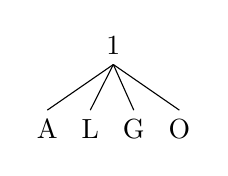
\begin{tikzpicture}
        \tikzset{every tree node/.style={align=center, anchor=north}}
        \Tree [.1 
                [.A ] 
                [.L ]
                [.G ]
                [.O ]
              ]
        \end{tikzpicture}
  \end{subfigure}
  \hfill
  \begin{subfigure}[b]{0.4\textwidth}
  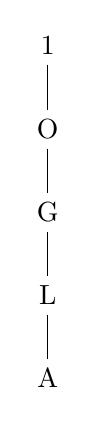
\begin{tikzpicture}
   \tikzset{every tree node/.style={align=center, anchor=north}}
            \Tree [.1 
        [.O 
            [.G 
                [.L 
                    [.A ] 
                ] 
            ] 
        ] 
]
    \end{tikzpicture}
  \end{subfigure}
\end{figure}
Die beiden Beispiele ergeben A, L, G, O, 1 in Postorder und $B^{\prime}$ ist nicht eindeutig.

\break

\section*{Aufgabe 2.3}
Ein Binärbaum hat die Eigenschaft, dass jeder Knoten höchstens 2 Kinder besitzt. Dieser wird als vollständig bezeichnet, wenn zusätzlich gilt, dass alle Blätter die gleiche Tiefe haben und jeder innere Knoten genau 2 Kinder besitzt. Beweisen oder widerlegen Sie folgende Aussagen:

\subsection*{a)}
Wenn $T$ ein Binärbaum mit $\left|V\right|$ Knoten ist, so besitzt $T$ genau $\left|V\right| - 1$ Kanten.

\subsection*{b)}
Jeder Binärbaum der Tiefe $t$ besitzt $^{t+1} - 1$ Knoten.

Gegenbeispiel: Wenn der Binärbaum nicht vollständig ist


\subsection*{c)}
Vollständige Binärbäume mit $\left|V\right|$ Knoten haben Tiefe $\log_2(\left|V\right| + 1) - 1$.

\begin{proof}[\unskip\nopunct]
uwu
\end{proof}

\break

\section*{Aufgabe 3.4}
Gegeben sei ein ungerichteter gewurzelter Baum $B = (V, E$) in Kind-Geschwister-Darstellung. Die Wurzel sei r.
Entwerfen Sie einen möglichst effizienten Algorithmus, der die Länge eines längsten einfachen Weges in B berechnet. Geben Sie Ihren Algorithmus in Pseudocode an, analysieren Sie seine Laufzeit und begründen Sie seine Korrektheit.


\begin{verbatim}
    function longest_path(node) {
        if node.child and node.sibling are none {
            height = temp_longest_path = 0
            return (height, temp_longest_path)

        } else if node.child is none but node.sibling exists {
            height, temp_longest_path = longest_path(node.sibling)
            if height == temp_longest_path == 0 {
                height += 1
                temp_longest_path += 1
            }

        } else if node.sibling is none but node.child exists {
            height, temp_longest_path = longest_path(node.child)
            height += 1
            temp_longest_path += 1

        } else if node.child and node.sibling exist {
            height_c, temp_longest_path_c = longest_path(node.child)
            height_s, temp_longest_path_s = longest_path(node.sibling)

            height = max(height_s, height_c + 1)
            path_parent = height_c + height_s + 3
            temp_longest_path = max(path_c, path_s, path_parent)
        }
        return (height, temp_longest_path)
    }
\end{verbatim}

Die Laufzeit des Algorithmus ist $\mathcal{O}(n^2)$, da es sich um eine Baumrekursion handelt und im Worst-case-Szenario die Funktion pro Rekursionsaufruf zwei mal Aufgerufen wird.\\

Bei den rekursiven Aufrufen kann es bei den Knoten zu den folgenden Szenarien kommen:

\begin{itemize}
    \item weder Kind noch Geschwister: der Knoten ist ein Blatt und der Elternknoten hat nur ein Kind. Die Höhe ist dann 0 und der längste Pfad über diesen Knoten bisher auch 0.
    \item kein Kind aber ein Geschwister: der Konten ist ein Blatt aber es geht beim Geschwister noch weiter. Da der Knoten selbst, als auch sein Geschwister mit dem gleichen Elternknoten verbunden ist, spielt es keine Rolle ob der Teilbaum des Geschwisterknoten am Knoten selbst sein kann. Wir übernehmen daher einfach nur die Werte die die Rekursion über den Geschwisterknoten zurückgibt.
    \item Wenn Kind aber kein Geschwister: die Anordnung der Knoten ist hier in einer einfachen Kette. Wir erhöhen die Höhe um 1 und den längsten Pfad um 1
    \item Wenn Kind und Geschwister: Der Entscheidungsfall. Hier treffen 2 Äste des Baums zusammen und der Algorithmus muss entscheiden was übernommen wird. Die Höhe ist einfach berechnet. Sie ist die größere Höhe der beiden Höhen $height\_c$ und $height\_s$. Der längste Weg ist komplexer. Wir berechnen hier den Weg vom tiefesten Blatt des Kind-Teilbaums zum tiefesten Blatt des Geschwister-Teilbaums. Da Zwischen dem Knoten selbst und dem Geschwisterknoten jedoch keine Kante vorliegt, müssen wir den Elternknoten dazunehmen. Wenn es einen Geschwisterknoten gibt, so gibt es automatisch auch einen Elternknoten. Somit addieren wir die beiden Höhen. Der Elternknoten muss jedoch auch noch im Weg miteinbezogen werden. Dei extra-Kanten sind dann vom Kind zum Knoten selbst, vom Knoten selbst zum Elternknoten und vom Elternknoten zum Geschwister. Daher die Konstante 3.
\end{itemize}




\break

\end{document}